\chapter{Fine-Tuning Techniques for Large Language Models}

\section{Overview of Fine-Tuning}

Large Language Models (LLMs) have demonstrated \textbf{extraordinary capabilities} in understanding, generating, and reasoning with natural language. This is largely due to their \textbf{pre-training on vast and diverse textual corpora} sourced from the internet, including books, articles, web pages, and forums. Through this process, models such as GPT, BERT, and LLaMA are able to capture a wide range of linguistic features—such as grammar, syntax, semantics—as well as broad factual and commonsense knowledge. These models operate as powerful general-purpose language processors that can be applied across a variety of tasks.

\vspace{0.5cm}

Despite these strengths, \textbf{pre-training alone is not sufficient} when it comes to achieving high performance on specialized tasks or domain-specific applications. For example, a general LLM might perform poorly on biomedical question answering, legal contract analysis, or technical customer support conversations. This limitation arises because the model, while broadly knowledgeable, may not be adequately exposed to the terminology, patterns, and nuances specific to these specialized fields during pre-training.

\vspace{0.5cm}

To bridge this gap, researchers and practitioners employ a technique known as \textbf{fine-tuning}. Fine-tuning refers to the process of \emph{continuing the training of a pre-trained model} on a smaller, curated dataset that is specific to a given task or domain. This dataset is typically labeled and reflects the desired outputs of the target application. During fine-tuning, the model adjusts its internal representations and decision boundaries to align more closely with domain-specific data, thereby improving its performance on the intended task.

\vspace{0.5cm}

Importantly, \textbf{fine-tuning enables the model to retain the general knowledge acquired during pre-training while specializing in a narrower objective}. This balance is critical: the model must not forget its foundational language capabilities, yet it must become more responsive and accurate in the new context. Tasks that benefit from fine-tuning include, but are not limited to, sentiment analysis, named entity recognition in specialized corpora (e.g., medical or financial texts), domain-specific dialogue systems, and document classification.


\vspace{1cm}

\begin{figure}[H]
    \centering
    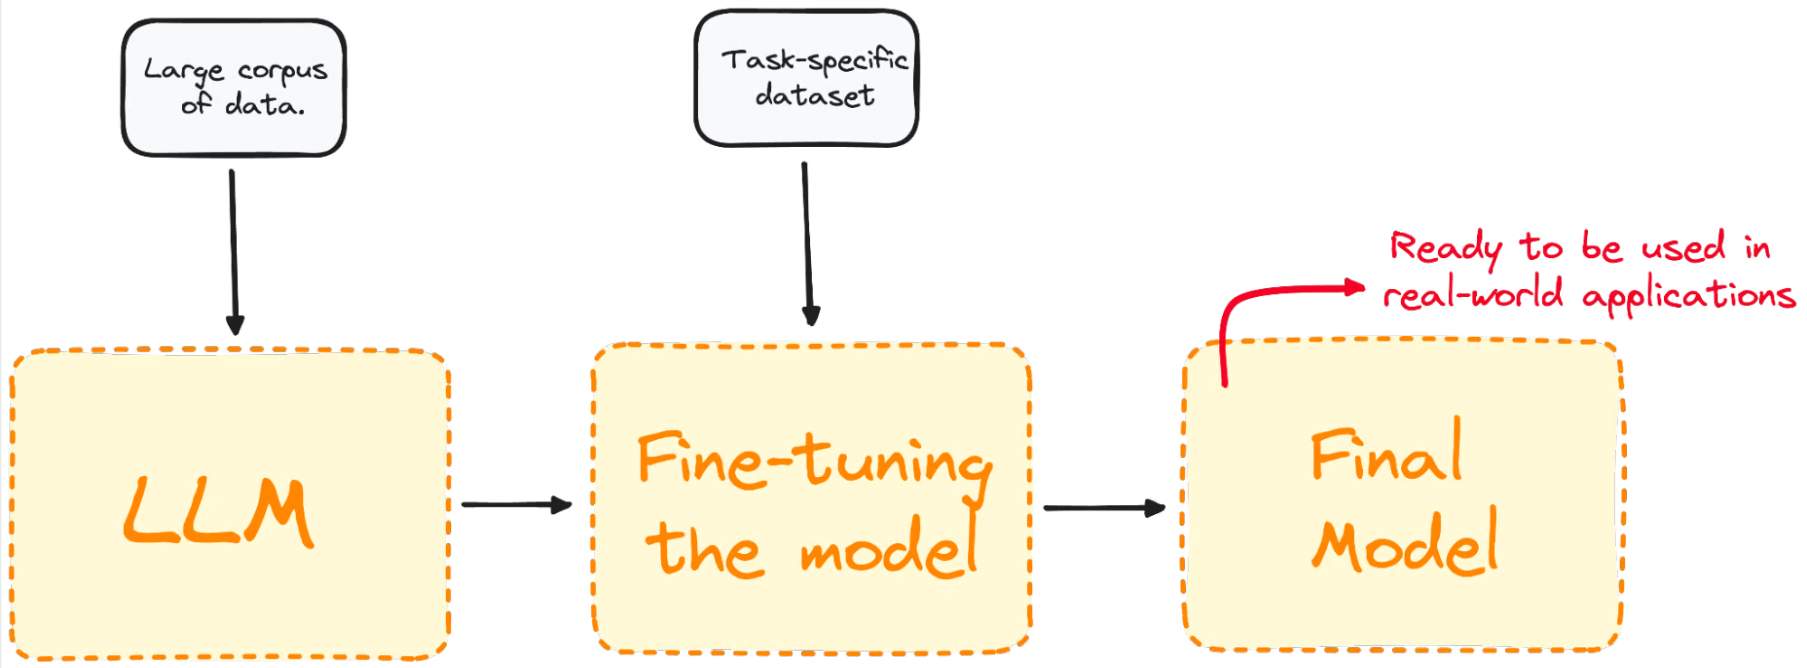
\includegraphics[width=0.95\linewidth]{img/chap05/5.1.2.png}
    \caption{From pre-trained LLM to final model ready for deployment through fine-tuning.}
    \label{fig:finetune_overview_2}
\end{figure}

\textbf{Fine-tuning is most commonly implemented using supervised learning}, in which a labeled dataset—consisting of input-output pairs specific to the target domain—is employed to guide the learning process. In this context, supervision refers to the use of explicit examples that show the model how to behave in the desired way. The objective is to refine the model’s outputs so that they become more relevant, accurate, and consistent with domain-specific expectations.

\vspace{0.5cm}

For example, a base LLM that was pre-trained on general-purpose internet text (e.g., Wikipedia, Common Crawl, news articles) may not perform optimally in specialized environments such as clinical report generation, legal document summarization, or customer service chatbots. By fine-tuning the base model on a \emph{proprietary knowledge base} or an \emph{application-specific dataset}—which may include domain-specific terminology, structured templates, or conversational patterns—the model's behavior becomes more aligned with the practical requirements of that particular context.

\vspace{0.5cm}

The \textbf{primary advantage of fine-tuning is its dual benefit}: it preserves the broad linguistic and factual knowledge acquired during the large-scale pre-training phase, while adapting the model to meet the unique demands of a specific application. This process results in a \textbf{fine-tuned model} that is more robust, task-aligned, and ready for integration into downstream systems. Such a model not only demonstrates improved quantitative performance (e.g., higher accuracy or F1 score) on the fine-tuned task but also offers greater utility in real-world deployments, where general-purpose responses may not suffice.

\vspace{0.5cm}

Figure~\ref{fig:finetune_overview_1} presents a high-level overview of this transformation pipeline: starting from a pre-trained base LLM, the model is enhanced via supervised fine-tuning on a specialized knowledge source. Likewise, Figure~\ref{fig:finetune_overview_2} illustrates a similar conceptual flow—from pre-training on a large generic corpus to targeted fine-tuning, ultimately producing a model that is \textbf{ready for deployment in real-world applications}.

\vspace{1cm}

\begin{figure}[H]
    \centering
    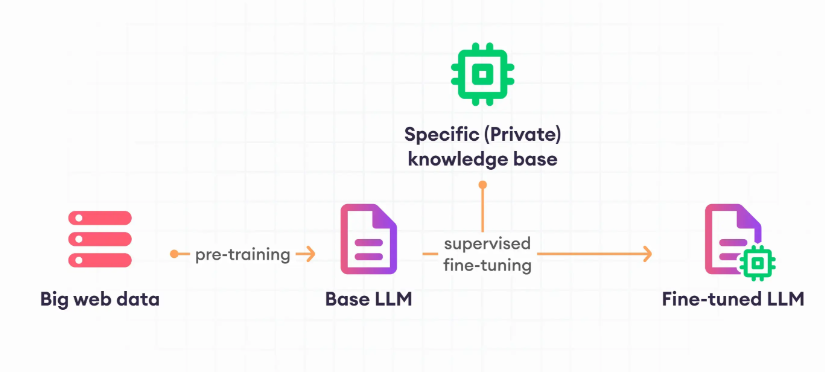
\includegraphics[width=0.85\linewidth]{img/chap05/5.1.1.png}
    \caption{Supervised fine-tuning of a base LLM using specific (possibly private) knowledge.}
    \label{fig:finetune_overview_1}
\end{figure}



\section{Types of Fine-Tuning Techniques}

\subsection{Full Fine-Tuning}
\begin{figure}[ht]
\centering
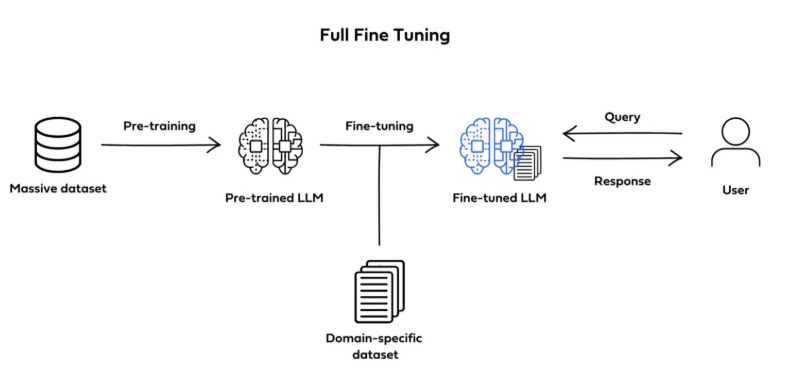
\includegraphics[width=0.9\textwidth]{img/chap05/5.2.1.png}
\caption{Illustration of the full fine-tuning process, showing how all parameters of a pre-trained LLM are updated using a domain-specific dataset to create a fine-tuned model that can handle specialized queries.}
\label{fig:full-fine-tuning}
\end{figure}

Full fine-tuning represents a comprehensive adaptation approach where \textbf{all parameters} of a pre-trained language model undergo adjustment using a task-specific or domain-specific dataset, as illustrated in Figure \ref{fig:full-fine-tuning}. This methodology leverages the foundational knowledge captured during pre-training while enabling the model to specialize for particular applications or domains.

\vspace{0.5cm}

In this approach, the entire neural network architecture—including attention mechanisms, feed-forward layers, and embedding matrices—is subjected to additional training iterations. The process begins with a pre-trained model that has already learned general language patterns and semantic relationships from massive corpora. This model serves as the initialization point for subsequent training, where every weight and bias throughout the network becomes eligible for modification.

\vspace{0.5cm}

The mechanism operates through supervised learning on labeled examples relevant to the target task. During fine-tuning, input sequences from the specialized dataset are processed through the model, generating predictions that are compared against ground truth labels. The resulting loss is backpropagated through the complete network hierarchy, and \textit{all parameters} are incrementally updated using optimization algorithms such as Adam or AdamW.

\vspace{0.5cm}

Mathematically, for each parameter $\theta_i$ in the model, updates follow the formula:
\begin{equation}
\theta_i^{new} = \theta_i^{old} - \eta \cdot \nabla_{\theta_i} \mathcal{L}
\end{equation}
where $\eta$ represents a carefully selected learning rate (typically smaller than in pre-training) and $\nabla_{\theta_i} \mathcal{L}$ denotes the gradient of the loss function with respect to parameter $\theta_i$.

\vspace{0.5cm}

To maintain stability during this process, practitioners typically implement learning rate scheduling, gradient accumulation, and normalization techniques. The learning trajectory often involves gradually decreasing the learning rate as fine-tuning progresses, allowing for initially substantial adaptations that become increasingly refined. Early stopping criteria based on validation performance help determine the optimal duration for fine-tuning iterations.

\vspace{0.5cm}

The computational workflow involves forward passes through the model for prediction generation, loss calculation against reference outputs, backward passes for gradient computation across all layers, and parameter updates according to the optimization algorithm's update rule. This cycle repeats for multiple epochs until convergence criteria are satisfied or a predetermined training budget is exhausted.

\vspace{0.5cm}

\subsection{Adapter-Based Fine-Tuning}
\begin{figure}[ht]
\centering
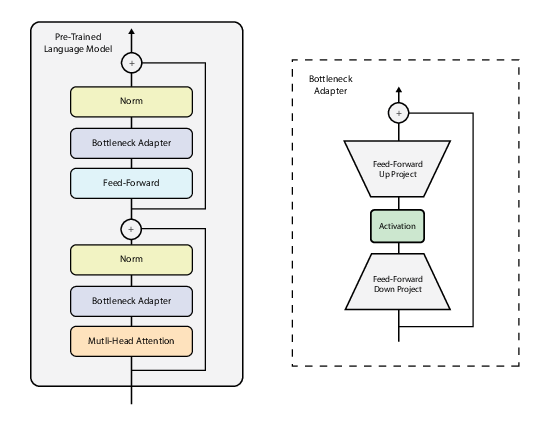
\includegraphics[width=0.9\textwidth]{img/chap05/5.2.2.png}
\caption{Architectural diagram of adapter-based fine-tuning showing the integration of bottleneck adapter modules within a pre-trained language model. The left panel illustrates adapter placement within the transformer architecture, while the right panel details the internal structure of a bottleneck adapter module.}
\label{fig:adapter-fine-tuning}
\end{figure}

Adapter-based fine-tuning represents an architectural modification approach that introduces compact, \textit{trainable neural modules}—known as adapters—into the layers of a pre-trained language model while maintaining the original model parameters in a \textbf{fixed state}. This methodology creates a parameter-efficient learning framework where only the newly inserted adapter components undergo weight updates during the adaptation process to task-specific requirements.

As depicted in Figure \ref{fig:adapter-fine-tuning}, adapter modules are strategically integrated at multiple points within the transformer architecture, typically following feed-forward networks and attention mechanisms in each layer. The fundamental structure of these adapters employs a bottleneck design that temporarily reduces dimensionality before restoring the original representation space.

\vspace{0.5cm}

The operational mechanism of an adapter module follows a three-stage computational pipeline. Initially, a down-projection matrix compresses the high-dimensional hidden representations from dimension $d$ to a significantly smaller bottleneck dimension $m$ (where $m \ll d$, often $m \approx d/64$ or smaller). Subsequently, a non-linear activation function—commonly GeLU (Gaussian Error Linear Unit) or ReLU (Rectified Linear Unit)—introduces non-linearity to the compressed representation. Finally, an up-projection matrix expands the processed features back to the original dimensionality $d$, allowing seamless integration with the surrounding network architecture.

\vspace{0.5cm}

Mathematically, for a hidden representation $h \in \mathbb{R}^d$ flowing through the network, the adapter transformation can be expressed as:

\begin{equation}
\text{Adapter}(h) = h + s \cdot (W_{\text{up}} \cdot f(W_{\text{down}} \cdot h + b_{\text{down}}) + b_{\text{up}})
\end{equation}

where $W_{\text{down}} \in \mathbb{R}^{m \times d}$ represents the down-projection matrix, $W_{\text{up}} \in \mathbb{R}^{d \times m}$ denotes the up-projection matrix, $b_{\text{down}} \in \mathbb{R}^m$ and $b_{\text{up}} \in \mathbb{R}^d$ are bias vectors, $f(\cdot)$ is the non-linear activation function, and $s$ is an optional scaling factor controlling the adapter's contribution magnitude.

\vspace{0.5cm}

The processing flow during inference or training involves the original model operations interspersed with adapter computations. Input embeddings traverse through the model's layers, with each layer's standard operations (self-attention, feed-forward networks, and normalization) occurring as designed in the pre-trained model. At designated insertion points, the adapter modules process and modify the representations through their bottleneck architecture while preserving the overall information flow via residual connections.

\vspace{0.5cm}

During the fine-tuning phase, optimization algorithms calculate gradients exclusively for the adapter parameters while treating the pre-trained model weights as constants. The learning process focuses on discovering optimal adapter configurations that effectively transform the pre-trained model's general-purpose representations into task-specialized features without altering the foundational knowledge encoded in the original parameters.

\vspace{0.5cm}

Different adapter variants may modify the precise insertion locations, bottleneck dimensionality, or employ parallel rather than sequential integration. Some implementations incorporate additional normalization layers within the adapter or utilize specialized initialization strategies to facilitate stable training dynamics.

\subsection{Low-Rank Adaptation (LoRA)}
\begin{figure}[ht]
\centering
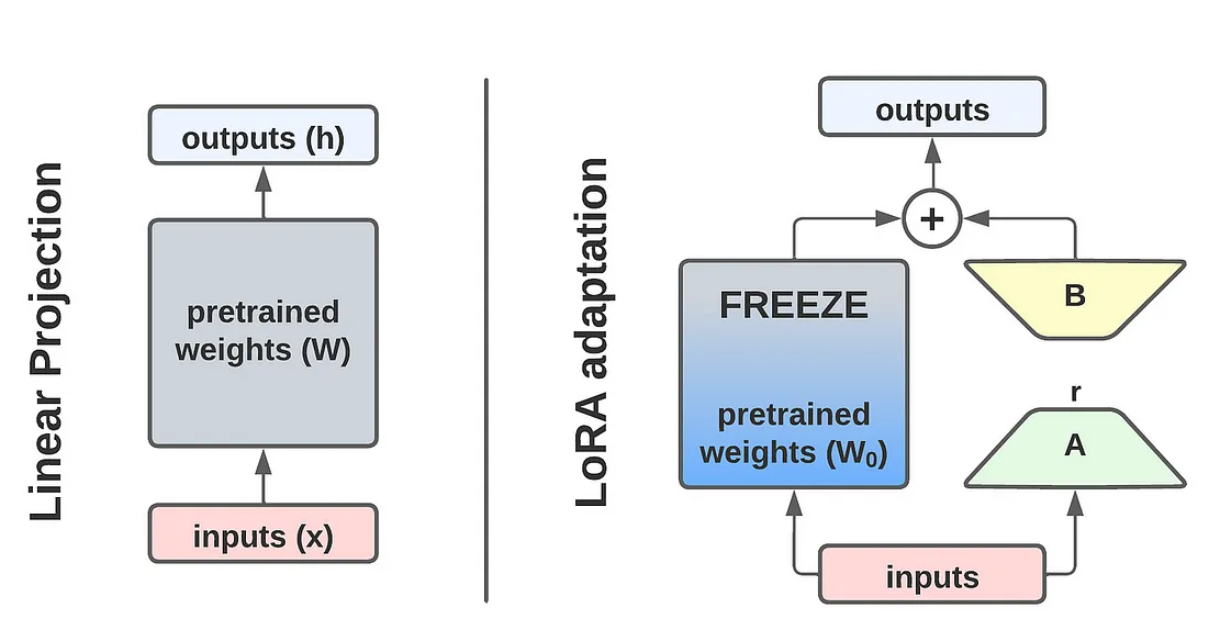
\includegraphics[width=0.9\textwidth]{img/chap05/5.2.3.png}
\caption{Comparison between standard linear projection (left) and Low-Rank Adaptation (right), illustrating how LoRA decomposes weight updates into low-rank matrices A and B that operate in parallel with frozen pre-trained weights.}
\label{fig:lora-adaptation}
\end{figure}

Low-Rank Adaptation (LoRA) represents an innovative approach to language model specialization that employs \textit{matrix decomposition principles} to enable efficient parameter updates while preserving the integrity of the original model architecture. This methodology, as depicted in Figure \ref{fig:lora-adaptation}, introduces trainable factorized matrices that operate alongside the \textbf{immutable pre-trained weights}, creating a parallel adaptation pathway.

LoRA builds upon the theoretical foundation that neural network weight updates during fine-tuning often exhibit low intrinsic dimensionality despite their high-dimensional parameterization. Rather than directly modifying the substantial weight matrices within transformer components, LoRA inserts decomposed rank-constrained matrices that capture task-specific adaptations while leaving original parameters untouched.

The mathematical formulation of LoRA centers on representing potential weight modifications through factorized low-rank structures. For a pre-trained weight matrix $W_0 \in \mathbb{R}^{d \times k}$ that would traditionally undergo updates during fine-tuning, LoRA introduces two smaller matrices: $A \in \mathbb{R}^{d \times r}$ and $B \in \mathbb{R}^{r \times k}$, where the rank hyperparameter $r$ is substantially smaller than both $d$ and $k$ (typically $r \in \{1, 2, 4, 8, 16, 32\}$). These matrices are initialized such that their product initially yields a zero contribution—$B$ is commonly initialized with zeros while $A$ uses Gaussian initialization.

During forward propagation through a LoRA-augmented network layer, the computation follows:

\begin{equation}
h' = W_0 x + \frac{\alpha}{r} A B x
\end{equation}

where $x$ represents the input activations, $h'$ denotes the output representation, $W_0$ signifies the frozen pre-trained weights, and $\alpha$ is a scaling hyperparameter that controls the magnitude of the adaptation contribution. The division by rank $r$ helps normalize the initial scale of the adapted outputs.

The learning process exclusively optimizes the parameters within matrices $A$ and $B$, leaving $W_0$ constant throughout training. Consequently, the effective update to the original transformation can be expressed as:

\begin{equation}
\Delta W = \frac{\alpha}{r} A B
\end{equation}

In practical implementations, LoRA modules are selectively applied to specific components within the transformer architecture. Most commonly, they target the query and value projection matrices within attention mechanisms, as these components heavily influence the contextual focus and information extraction capabilities of the model. Some implementations extend this approach to include key projections and feed-forward network weights, with each application following the same fundamental low-rank principle.

The computational workflow involves channeling input activations through both the original frozen pathway and the parallel LoRA pathway. The outputs from both routes are then additively combined before proceeding to subsequent operations in the network. This parallel processing structure means that during inference, the LoRA matrices can be merged with the original weights by computing $W = W_0 + \frac{\alpha}{r} A B$, enabling efficient deployment without architectural modifications.

At a system level, different LoRA modules can be trained for various tasks or domains while sharing the same underlying frozen model. The training procedure follows standard optimization approaches but isolates gradient computation and parameter updates to exclusively affect the low-rank components, maintaining the constrained adaptation space throughout the fine-tuning process.

\subsection{Prefix-Tuning}
Prefix-tuning represents an \textit{innovative} parameter-efficient fine-tuning method that modifies the behavior of a pre-trained language model by prepending a small sequence of trainable continuous vectors—called \textbf{prefix parameters}—to the input of each Transformer layer. This approach enables task-specific adaptation while keeping the underlying parameters of the language model completely \textbf{frozen}; only the prefix parameters are updated during the training process.

\begin{figure}[t]
\centering
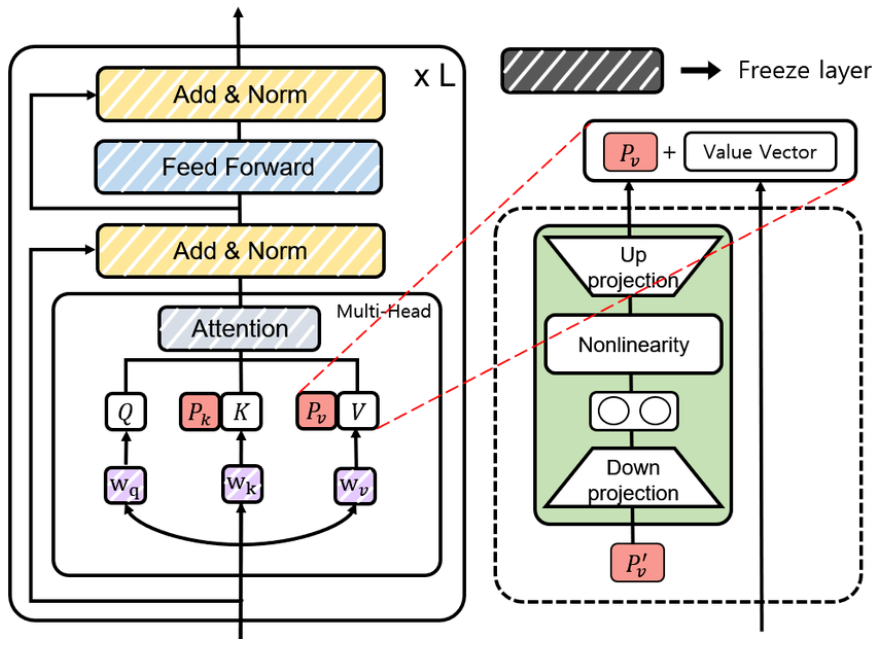
\includegraphics[width=\linewidth]{img/chap05/5.2.4.png}
\caption{Architecture of prefix-tuning. The left side shows the overall Transformer structure with attention and feed-forward blocks repeated L times. The right side illustrates the prefix mechanism, where trainable prefix vectors $P_K$ and $P_V$ are prepended to keys and values in the attention mechanism. The prefix undergoes reparameterization through a small MLP with up-projection, nonlinearity, and down-projection steps before being added to the attention computation.}
\label{fig:prefix_tuning}
\end{figure}

In the standard implementation, instead of optimizing the entire model's parameter space, prefix-tuning learns task-specific key and value vectors that are \textit{concatenated} to the original self-attention mechanism. For a Transformer block at layer \( l \), the attention computation is modified as follows:
\[
\text{Attention}(Q, [P_K^l; K], [P_V^l; V])
\]
where \( P_K^l \) and \( P_V^l \) represent the learned prefix key and value vectors for layer \( l \), and \( Q, K, V \) are the original query, key, and value matrices derived from the input tokens.

These prefix vectors function as \textbf{soft prompts}—learned continuous embeddings that effectively guide the model's behavior—without altering the model's original weights. The prefixes are typically initialized randomly and subsequently optimized using standard backpropagation techniques when trained on a supervised downstream task.

As illustrated in Figure \ref{fig:prefix_tuning}, the prefix vectors undergo a reparameterization process through a small MLP network containing an up-projection layer, a nonlinearity function, and a down-projection layer. This reparameterization helps stabilize the training dynamics and improves optimization efficiency. The resulting prefix parameters $P_K$ and $P_V$ are then prepended to the key and value matrices in the multi-head attention mechanism, effectively conditioning the model's predictions without modifying its core parameters.

The prefix-tuning mechanism operates across all layers of the Transformer architecture, with each layer receiving its own set of trainable prefix vectors. This multi-layer conditioning allows the prefixes to influence both lower-level features (in earlier layers) and higher-level semantic representations (in later layers), providing comprehensive control over the model's behavior while maintaining the underlying pre-trained knowledge intact.

\subsection{Prompt-Tuning}
Prompt-tuning represents a \textit{streamlined} and parameter-efficient fine-tuning strategy where a small number of \textbf{trainable continuous token embeddings} are prepended to the input sequence of a pre-trained language model. Unlike prefix-tuning, which modifies representations at multiple internal layers, prompt-tuning exclusively affects the initial input embedding layer, maintaining the entire underlying model architecture and parameters \textbf{completely frozen}.

\begin{figure}[t]
\centering
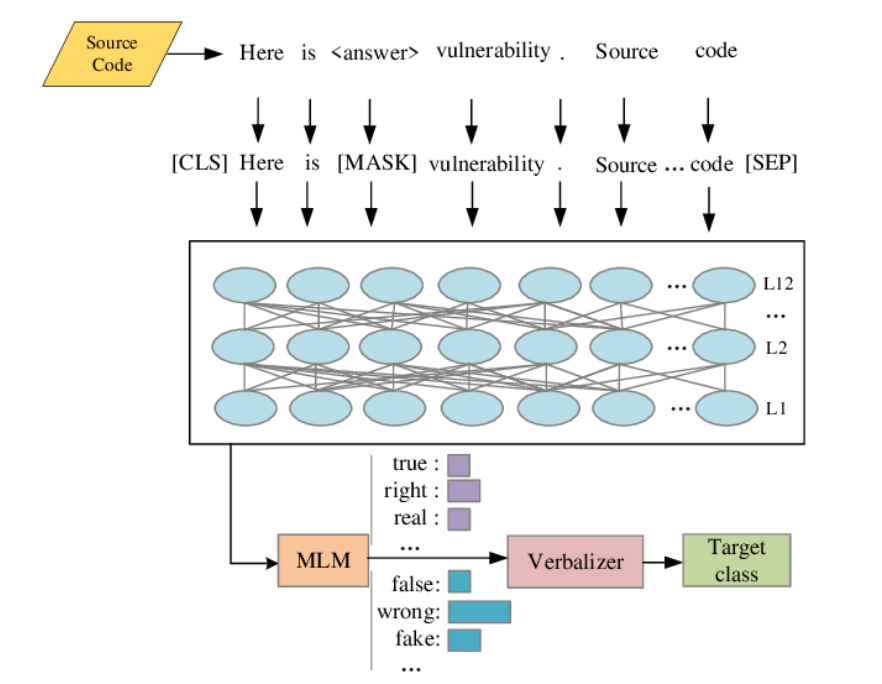
\includegraphics[width=0.8\linewidth]{img/chap05/5.2.5.png}
\caption{Architecture of prompt-tuning for classification tasks. The continuous soft prompts are prepended to tokenized inputs at the embedding layer. Special tokens like [CLS], [MASK], and [SEP] maintain their functionality while the model processes both the soft prompts and regular input through its layers (L1 through L12). The output is then processed by a masked language model (MLM) head and verbalizer to produce the target classification.}
\label{fig:prompt_tuning}
\end{figure}

In the prompt-tuning framework, the language model processes a modified input sequence represented as:
\[
[\mathbf{P}_1, \mathbf{P}_2, \ldots, \mathbf{P}_m, x_1, x_2, \ldots, x_n]
\]
where \( \mathbf{P}_i \in \mathbb{R}^d \) are the \textit{learnable} soft prompt embeddings that exist in the same dimensional space as the model's vocabulary embeddings, and \( x_i \) are the embeddings of the original input tokens. Crucially, these prompt vectors are not tied to actual vocabulary tokens but are free to occupy any position in the embedding space.

As illustrated in Figure \ref{fig:prompt_tuning}, the continuous prompt vectors are concatenated with the standard token embeddings at the input level. The combined sequence then flows through the Transformer layers (L1 through L12) without any modifications to the model architecture. The original source input undergoes tokenization with appropriate special tokens (e.g., [CLS], [MASK], [SEP] for BERT-based models) before being combined with the soft prompts.

During the training process, only the parameters of these continuous prompt embeddings are optimized, while keeping all pre-trained model weights fixed. The prompt vectors learn to elicit the desired behavior from the frozen language model through standard backpropagation based on task-specific loss functions. This creates a form of implicit conditioning that guides the model's predictions toward the target task.

For classification tasks specifically, as shown in the diagram, the processed sequence typically passes through a masked language modeling (MLM) head, followed by a verbalizer component that maps the model's vocabulary distribution to target class labels. The verbalizer establishes connections between the model's output probabilities for words like "true," "right," and "real" versus "false," "wrong," and "fake" to produce the final classification decision.

The continuous prompt embeddings are typically initialized randomly or from embeddings of template tokens and then optimized through gradient descent. The optimization process effectively discovers prompt representations that maximize task performance by leveraging the frozen model's pre-trained knowledge, allowing it to produce appropriate outputs without modifying its internal parameters.

\subsection{Instruction Tuning}
Instruction tuning is a specialized fine-tuning methodology in which a pre-trained language model undergoes additional training on a diverse collection of examples formatted as \textbf{explicit natural language directives paired with appropriate responses}. The fundamental principle involves aligning the model's behavior with human intentions by teaching it to interpret and follow clearly articulated prompts such as: \textit{"Translate the following sentence into French,"} \textit{"Summarize the paragraph below,"} or \textit{"Explain the concept of quantum computing to a high school student."} 

\begin{figure}[t]
\centering
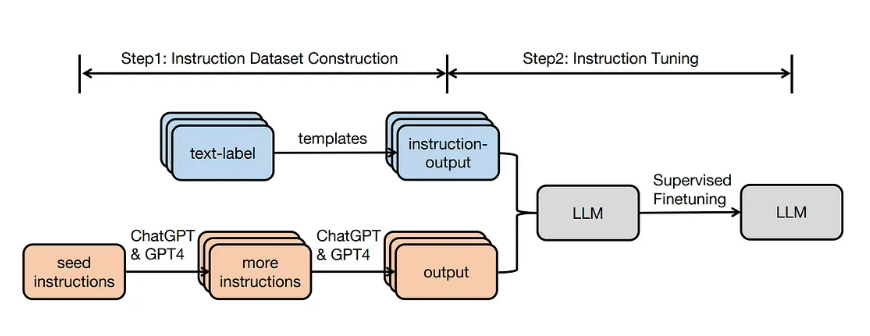
\includegraphics[width=\linewidth]{img/chap05/5.2.6.png}
\caption{The two-stage process of instruction tuning. Step 1 (left) illustrates the instruction dataset construction, where text-label templates and seed instructions are expanded using stronger models like ChatGPT and GPT-4 to generate diverse instruction-output pairs. Step 2 (right) shows the actual instruction tuning phase, where the constructed dataset is used to perform supervised fine-tuning on the target LLM.}
\label{fig:instruction_tuning}
\end{figure}

As depicted in Figure \ref{fig:instruction_tuning}, the instruction tuning process typically consists of two distinct phases: instruction dataset construction and supervised fine-tuning. In the dataset construction phase, developers create or curate a wide range of instruction-output pairs, often using larger, more capable models (such as ChatGPT and GPT-4) to generate diverse examples from seed instructions and text-label templates. This approach enables the creation of comprehensive instruction datasets spanning numerous domains and task types.

During the instruction tuning phase, the training data consists of structured \textit{(instruction, input, output)} triplets. Each training example typically follows a consistent format:
\[
\texttt{Instruction:}~\textit{Perform task X} \quad \texttt{Input:}~\textit{Relevant data or query} \quad \texttt{Output:}~\textit{Expected response}
\]
For simpler tasks, the format may be condensed to instruction-output pairs where the input is implicitly contained within the instruction itself.

In the training procedure, the model receives the concatenation of the instruction and input (when present) and is trained using standard language modeling objectives to generate the target output. This supervised learning process utilizes traditional optimization techniques such as gradient descent with cross-entropy loss, maximizing the likelihood of producing the expected responses given the instructions.

The learning mechanism enables the model to establish connections between linguistic formulations of tasks and the corresponding expected behaviors. As the model processes numerous instruction-output examples across diverse domains, it gradually develops a generalized capability to interpret new instructions—even those formulated differently from what it encountered during training—and produce appropriate responses based on its understanding of the task requirements.

Unlike parameter-efficient methods such as prompt-tuning that incorporate learned continuous embeddings, instruction tuning directly modifies the model's full parameter space through conventional fine-tuning. This comprehensive parameter update enables the model to internalize instruction-following behavior across its entire network architecture, rather than concentrating adaptations in specific components.

The instruction tuning paradigm represents a significant shift from earlier approaches that required task-specific fine-tuning or elaborate prompt engineering. By teaching models to respond appropriately to natural language instructions, this method bridges the gap between how humans communicate their intentions and how AI systems interpret and execute tasks.


\subsection{Reinforcement Learning from Human Feedback (RLHF)}
Reinforcement Learning from Human Feedback (RLHF) represents a \textit{sophisticated} multi-stage fine-tuning paradigm designed to align large language models with human preferences and values. Unlike conventional training approaches that rely exclusively on supervised learning with predefined datasets, RLHF incorporates direct human evaluations into the optimization process, enabling models to generate outputs that better reflect human judgments of quality, helpfulness, and appropriateness.

\begin{figure}[t]
\centering
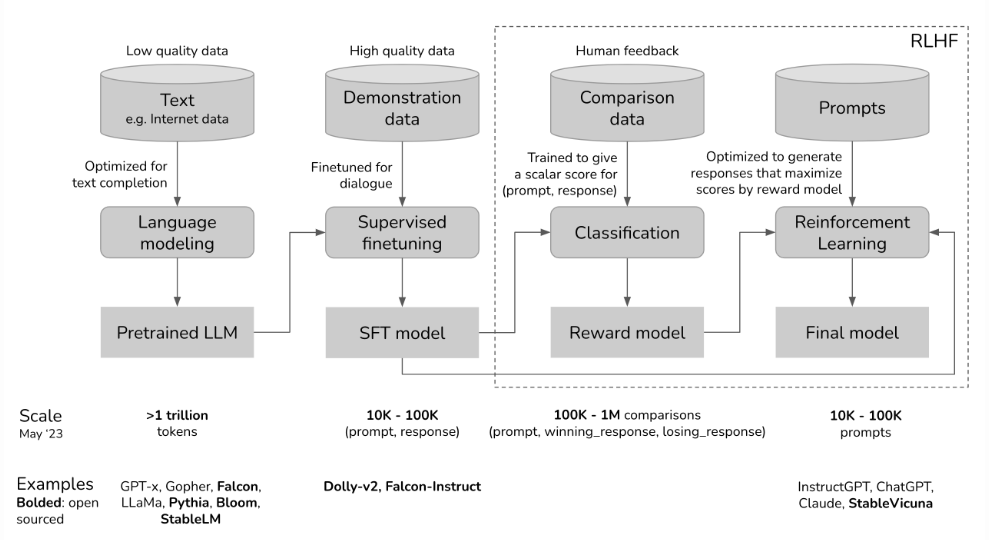
\includegraphics[width=\linewidth]{img/chap05/5.2.7.png}
\caption{Complete RLHF training pipeline. The process begins with pretraining on large text corpora (left), followed by supervised fine-tuning on demonstration data. The RLHF-specific components (outlined by the dashed box) include reward model training from human comparison data and reinforcement learning optimization. The figure also shows typical data scales for each stage and examples of models that have used these techniques.}
\label{fig:rlhf_pipeline}
\end{figure}

As illustrated in Figure \ref{fig:rlhf_pipeline}, the RLHF methodology consists of a sequential pipeline with several distinct phases, each building upon the previous one:

\begin{enumerate}
    \item \textbf{Supervised Fine-Tuning (SFT):} The process begins with a pre-trained language model that has already acquired broad linguistic capabilities through exposure to vast amounts of text data (typically exceeding 1 trillion tokens). This foundation model undergoes initial adaptation through supervised fine-tuning on a curated dataset of \textit{high-quality demonstrations}—typically comprising 10,000 to 100,000 prompt-response pairs. These examples often consist of carefully crafted responses that exhibit desirable characteristics such as helpfulness, accuracy, and safety. The resulting SFT model serves as the starting point for subsequent preference-based optimization.
    
    \item \textbf{Reward Model Development:} In this critical stage, a separate \textbf{evaluative model} is trained to predict human preferences regarding language model outputs. Human annotators are presented with a prompt and multiple alternative responses (typically generated by the SFT model) and asked to rank or compare them based on quality criteria. These comparative judgments—ranging from 100,000 to 1 million comparisons—form a specialized dataset of triplets (prompt, winning\_response, losing\_response) or (prompt, response, score). The reward model learns to assign scalar values to responses that correlate with human preferences, essentially distilling human judgments into a computational form that can guide optimization.
    
    \item \textbf{Reinforcement Learning Optimization:} The final phase leverages the trained reward model to further refine the SFT model through reinforcement learning techniques—most commonly \textit{Proximal Policy Optimization (PPO)}. During this process, the language model (now functioning as a policy) generates responses to a diverse set of prompts (typically 10,000 to 100,000). Each generated response receives a scalar reward score from the reward model, which serves as the optimization signal. The language model parameters are iteratively updated to maximize these reward scores while maintaining reasonable proximity to the original SFT model to preserve linguistic capabilities and prevent pathological optimization behaviors.
\end{enumerate}

From a mathematical perspective, the reinforcement learning objective can be formulated as maximizing:
\[
\mathbb{E}_{y \sim \pi_\phi(y|x)}[R_\theta(x, y) - \beta \log(\pi_\phi(y|x)/\pi_{\text{SFT}}(y|x))]
\]
where \( \pi_\phi \) represents the policy (language model) being optimized with parameters \( \phi \), \( R_\theta \) denotes the reward model with parameters \( \theta \), \( x \) is the input prompt, \( y \) is the generated response, and \( \pi_{\text{SFT}} \) is the initial supervised fine-tuned model. The second term—controlled by the hyperparameter \( \beta \)—constitutes a KL-divergence penalty that prevents the optimized model from deviating too drastically from the SFT model.

The RLHF framework essentially creates a feedback loop where human preferences guide model optimization through an automated reward mechanism. This methodology enables language models to generate responses that increasingly align with human expectations and values across a diverse range of tasks and interactions. By incorporating direct human feedback into the training process, RLHF addresses fundamental challenges in specifying complex objectives that are difficult to articulate through conventional loss functions or supervised learning approaches alone.

\section{Advantages and Disadvantages of Fine-Tuning Methods}

\subsection{Full Fine-Tuning}

Full fine-tuning involves updating all parameters of a pre-trained language model when adapting it to a downstream task. This comprehensive approach offers distinct trade-offs that practitioners should consider.

\subsubsection{Advantages}
\begin{itemize}
    \item \textbf{Superior Performance}: Generally achieves the highest task-specific performance compared to parameter-efficient methods, as all model weights can adapt to the target domain.
    \item \textbf{Complete Representation Learning}: Allows modification of features at all levels of abstraction throughout the network hierarchy.
    \item \textbf{Robust Transfer}: Can effectively adapt to domains significantly different from pre-training data by thoroughly rewriting relevant representations.
    \item \textbf{Flexibility}: Imposes no architectural constraints on adaptation, enabling unrestricted optimization.
\end{itemize}

\subsubsection{Disadvantages}
\begin{itemize}
    \item \textbf{Resource Intensity}: Requires substantial computational resources (GPU/TPU memory and compute) proportional to the model size.
    \item \textbf{Storage Overhead}: Each fine-tuned variant requires storing a complete copy of model parameters, creating significant storage costs for large models.
    \item \textbf{Catastrophic Forgetting}: Models may lose general capabilities and knowledge acquired during pre-training when aggressively optimized on narrow tasks.
    \item \textbf{Overfitting Risk}: Higher susceptibility to overfitting on smaller datasets due to the large number of trainable parameters.
\end{itemize}

\subsubsection{Practical Considerations}
Full fine-tuning is most appropriate when maximum task performance is the primary objective and sufficient computational resources are available. Consider alternatives when facing computational constraints or working with limited datasets. For implementation, use smaller learning rates than during pre-training (typically 1e-5 to 1e-6), apply appropriate regularization techniques, and monitor for signs of catastrophic forgetting. Mixed-precision training and gradient checkpointing can help reduce memory requirements for larger models.

\subsection{Adapter-Based Fine-Tuning}

Adapter-based fine-tuning introduces small, trainable modules (adapters) between layers of a pre-trained language model while keeping the original parameters frozen. This parameter-efficient approach offers a distinct set of trade-offs for downstream task adaptation.

\subsubsection{Advantages}
\begin{itemize}
\item \textbf{Parameter Efficiency}: Only a small fraction of parameters (typically 1-4% of the full model) are trainable, drastically reducing memory requirements.
\item \textbf{Modular Design}: Enables easy swapping of task-specific adapters without modifying the base model, facilitating multi-task learning.
\item \textbf{Preserved Pretrained Knowledge}: The frozen base model retains its original capabilities, minimizing catastrophic forgetting.
\item \textbf{Scalability}: Particularly effective for very large models where full fine-tuning would be prohibitive.
\item \textbf{Fast Deployment}: Multiple adapters can be stored and loaded efficiently compared to full model copies.
\end{itemize}

\subsubsection{Disadvantages}
\begin{itemize}
\item \textbf{Performance Trade-off}: May achieve slightly lower task performance compared to full fine-tuning, particularly on complex tasks.
\item \textbf{Architectural Constraints}: Requires careful design of adapter placement and dimensionality within the network.
\item \textbf{Inference Overhead}: Introduces additional computational layers during forward passes, though typically minimal.
\item \textbf{Task-Specialization Limits}: May struggle with domain shifts that require deeper modifications to base representations.
\end{itemize}

\subsubsection{Practical Considerations}
Adapter-based approaches are ideal when computational resources are limited, when preserving base model capabilities is crucial, or when managing multiple task-specific versions. Optimal implementation involves:
\begin{itemize}
\item Strategic placement of adapters (typically after attention and FFN layers)
\item Careful tuning of adapter dimensionality (bottleneck size)
\item Potential combination with prefix tuning or other parameter-efficient methods
\item Use of adapter composition techniques for multi-task scenarios
\end{itemize}
Recent variants like \texttt{LoRA} (Low-Rank Adaptation) and parallel adapters offer additional design choices worth considering based on specific application requirements.

\subsection{Low-Rank Adaptation (LoRA)}

Low-Rank Adaptation (LoRA) is a parameter-efficient fine-tuning method that injects trainable low-rank matrices into a pre-trained model while keeping the original weights frozen. This approach achieves efficient adaptation with minimal memory overhead by decomposing weight updates into low-rank components.

\subsubsection{Advantages}
\begin{itemize}
    \item \textbf{Parameter Efficiency}: Updates only a small subset of parameters (typically <1\% of the full model), drastically reducing memory and storage costs while avoiding the need to store multiple full-model checkpoints.
    
    \item \textbf{No Inference Latency}: Unlike adapters, LoRA can be merged with the original weights after training, introducing zero additional computation during inference.
    
    \item \textbf{Preserved Pretrained Knowledge}: The base model remains frozen, minimizing catastrophic forgetting and enabling switching between different task-specific LoRA modules without reloading the base model.
    
    \item \textbf{Scalability}: Particularly effective for fine-tuning large language models (LLMs) where full fine-tuning is impractical, and compatible with quantization techniques for further efficiency gains.
    
    \item \textbf{Flexibility}: Can be applied selectively to specific layers (e.g., attention weights only) for targeted adaptation.
\end{itemize}

\subsubsection{Disadvantages}
\begin{itemize}
    \item \textbf{Performance Trade-off}: May underperform full fine-tuning on tasks requiring deep architectural changes due to the low-rank constraint limiting update expressiveness.
    
    \item \textbf{Rank Selection Sensitivity}: Performance depends on choosing an appropriate rank for the decomposition (too low leads to weak adaptation, too high has diminishing returns).
    
    \item \textbf{Task-Specific Tuning Required}: Optimal rank and layer selection may vary across tasks, requiring experimentation.
    
    \item \textbf{Limited Extreme Domain Adaptation}: Less effective than full fine-tuning for highly specialized domains needing fundamental representation changes.
\end{itemize}

\subsubsection{Practical Considerations}
LoRA is best suited when:
\begin{itemize}
    \item Resource efficiency is a priority (e.g., fine-tuning on consumer-grade GPUs)
    \item Multiple task-specific adaptations need efficient storage and deployment
    \item Minimal inference overhead is required
\end{itemize}


\subsection{Prefix-Tuning}

Prefix-tuning is a parameter-efficient fine-tuning method that prepends trainable continuous vectors (prefixes) to the hidden states in transformer layers while keeping the original model parameters frozen. This approach provides task-specific adaptation through learned "soft prompts" that condition the model's behavior.

\subsubsection{Advantages}
\begin{itemize}
    \item \textbf{Extreme Parameter Efficiency}: Only requires training of a small prefix (typically 0.1-1\% of model parameters), making it highly memory-efficient.
    
    \item \textbf{Architectural Preservation}: Maintains the original model architecture without modifications, ensuring no inference overhead after deployment.
    
    \item \textbf{Multi-Task Flexibility}: Different prefixes can be swapped in/out at runtime, enabling efficient multi-task serving from a single base model.
    
    \item \textbf{Knowledge Retention}: Frozen base model parameters prevent catastrophic forgetting of pre-trained knowledge.
    
    \item \textbf{Discrete Prompt Generalization}: Outperforms manual prompt engineering by learning optimal continuous prefixes.
\end{itemize}

\subsubsection{Disadvantages}
\begin{itemize}
    \item \textbf{Sequence Length Impact}: Added prefix tokens reduce the available context window for the actual input.
    
    \item \textbf{Optimization Challenges}: Requires careful tuning of prefix length and learning rates due to the discrete nature of the approach.
    
    \item \textbf{Performance Trade-offs}: May underperform full fine-tuning on complex tasks requiring deep architectural changes.
    
    \item \textbf{Layer Placement Sensitivity}: Performance varies significantly based on which transformer layers receive prefixes.
\end{itemize}

\subsubsection{Practical Considerations}
Prefix-tuning is most appropriate when parameter efficiency and model preservation are prioritized over absolute task performance, particularly in resource-constrained environments or multi-task scenarios. Consider alternative methods when working with tasks requiring fundamental architectural changes or when the prefix length would excessively reduce the available context window. For implementation, use moderate learning rates (typically 1e-4 to 1e-5) given the discrete nature of prefix optimization, apply layer normalization to the prefixes for training stability, and carefully tune the prefix length based on task complexity. Techniques like gradient clipping and weight decay are particularly important for successful optimization. The approach works especially well when combined with prompt-based fine-tuning paradigms.

\subsection{Prompt-Tuning}

Prompt-tuning is a parameter-efficient approach that learns continuous "soft" prompts while keeping the entire pre-trained model frozen. Unlike traditional prompt engineering, it automatically optimizes task-specific embeddings prepended to the input sequence.

\subsubsection{Advantages}
\begin{itemize}
    \item \textbf{Extreme Efficiency}: Only requires training the prompt parameters (typically <0.1\% of model parameters), making it highly resource-friendly.
    
    \item \textbf{No Architecture Changes}: Preserves the original model structure without adding new layers or modules.
    
    \item \textbf{Multi-Task Deployment}: Enables serving multiple tasks from a single frozen model by switching learned prompts.
    
    \item \textbf{Knowledge Preservation}: Maintains all original model capabilities as base parameters remain frozen.
    
    \item \textbf{Superior to Manual Prompts}: Outperforms hand-crafted discrete prompts through learned continuous representations.
\end{itemize}

\subsubsection{Disadvantages}
\begin{itemize}
    \item \textbf{Context Window Reduction}: Learned prompts consume part of the available sequence length.
    
    \item \textbf{Task Complexity Limitations}: Less effective for tasks requiring substantial model adaptation beyond input conditioning.
    
    \item \textbf{Optimization Sensitivity}: Requires careful tuning of prompt length and learning rates.
    
    \item \textbf{Performance Gap}: Generally underperforms full fine-tuning on complex downstream tasks.
\end{itemize}

\subsubsection{Practical Considerations}
Prompt-tuning is most suitable when working with very large models where parameter efficiency is crucial, or when maintaining the base model's general capabilities is essential. Consider alternative methods when dealing with tasks that require significant architectural changes or when the performance gap is unacceptable. For implementation, use relatively high learning rates (typically 1e-3 to 1e-4) due to the small parameter count, initialize prompts from relevant word embeddings when possible, and experiment with prompt lengths between 20-100 tokens based on task complexity. The approach works particularly well when combined with few-shot learning paradigms.

\subsection{Instruction Tuning}

Instruction tuning is a supervised fine-tuning approach that trains language models on diverse tasks formatted with natural language instructions, enabling zero-shot generalization to unseen tasks. This method focuses on teaching models to follow task specifications rather than specializing for particular datasets.

\subsubsection{Advantages}
\begin{itemize}
    \item \textbf{Zero-shot Generalization}: Enables models to perform unseen tasks by following natural language instructions without task-specific fine-tuning.
    
    \item \textbf{Task Formulation Flexibility}: Handles diverse tasks through standardized instruction-input-output formatting.
    
    \item \textbf{Human-Aligned Behavior}: Produces more interpretable and controllable outputs by conditioning on explicit instructions.
    
    \item \textbf{Multi-Task Efficiency}: Single instruction-tuned model can replace multiple specialized models.
    
    \item \textbf{Knowledge Preservation}: Maintains broad capabilities from pre-training while adding instruction-following skills.
\end{itemize}

\subsubsection{Disadvantages}
\begin{itemize}
    \item \textbf{Data Requirements}: Needs large, diverse collections of instruction-output pairs covering various task types.
    
    \item \textbf{Training Cost}: Requires substantial computational resources comparable to full fine-tuning.
    
    \item \textbf{Instruction Sensitivity}: Performance heavily depends on how tasks are formulated in natural language.
    
    \item \textbf{Over-optimization Risk}: May lose general capabilities if tuned too aggressively on narrow instruction sets.
\end{itemize}

\subsubsection{Practical Considerations}
Instruction tuning is most valuable when building general-purpose models that need to handle diverse, unpredictable tasks through natural language interaction. It becomes particularly effective when paired with large language models that have sufficient capacity to internalize the instruction-following paradigm. The approach requires careful curation of training tasks to ensure broad coverage of potential use cases, with special attention to the variety and clarity of instruction formulations. While powerful for zero-shot applications, performance on specific tasks may still lag behind specialized fine-tuned models, making the technique better suited for general assistants than domain-specific applications where peak performance is required.

\subsection{Reinforcement Learning from Human Feedback (RLHF)}

RLHF is an alignment technique that uses reinforcement learning to fine-tune language models based on human preferences, typically through a reward model trained on human judgments. This approach bridges the gap between raw language model capabilities and human-desirable behaviors.

\subsubsection{Advantages}
\begin{itemize}
    \item \textbf{Human-Aligned Outputs}: Produces responses better aligned with human values and preferences compared to supervised fine-tuning alone.
    
    \item \textbf{Complex Behavior Shaping}: Can optimize for nuanced aspects of responses (e.g., helpfulness, harmlessness) that are difficult to specify explicitly.
    
    \item \textbf{Adaptability}: Capable of learning from relatively small amounts of human preference data compared to the original training data.
    
    \item \textbf{Multi-Dimensional Optimization}: Enables balancing of competing objectives through reward modeling.
    
    \item \textbf{Iterative Improvement}: Supports continuous refinement of model behavior through additional feedback rounds.
\end{itemize}

\subsubsection{Disadvantages}
\begin{itemize}
    \item \textbf{Implementation Complexity}: Requires sophisticated pipeline with reward modeling and RL optimization components.
    
    \item \textbf{High Resource Demands}: Needs substantial compute for both reward model training and RL fine-tuning phases.
    
    \item \textbf{Reward Hacking Risk}: Models may exploit weaknesses in the reward model rather than genuinely improving.
    
    \item \textbf{Data Bottleneck}: Quality heavily depends on the quantity and diversity of human preference data.
    
    \item \textbf{Instability}: RL training can be unpredictable and sensitive to hyperparameters.
\end{itemize}

\subsubsection{Practical Considerations}
RLHF is most valuable when aligning large language models to complex human preferences where simple supervised approaches are insufficient. The technique proves particularly effective for refining safety properties and conversational abilities, but requires careful implementation to avoid reward gaming behaviors. Significant investment in high-quality human preference data collection is essential, and the approach works best when combined with initial supervised fine-tuning as a foundation. While powerful, RLHF should be deployed judiciously due to its computational demands and implementation complexity, making it most suitable for foundational models rather than application-specific tuning.

\newpage 
